\chapter{Existing Site Conditions}
\label{ch:fscf-site-cond}


The SDSTA currently operates and maintains the Sanford Underground Research Facility (SURF) at the former Homestake mine in Lead, South Dakota. The SURF property comprises 186 acres on the surface and 7,700 acres underground. The SURF Surface Campus includes approximately 253,000 gross square feet (gsf) of existing structures. Using a combination of private funds through T. Denny Sanford, South Dakota Legislature-appropriated funding, and a federal Department of Housing and Urban Development (HUD) Grant, the SDSTA has made significant progress in stabilizing and rehabilitating the SURF facility to provide for safe access and prepare the site for new laboratory construction. These efforts have included dewatering of the underground facility and mitigating and reducing risks %independent of \
\fixme{beyond those identified in the (year) assessment of the existing facility conditions done for (this needs some context)} the former Deep Underground Science and Engineering Laboratory (DUSEL).
% efforts and funding. 

Figure~\ref{fig:regional-context} shows SURF's location within the region as a part of the northern Black Hills of South Dakota. Figure~\ref{fig:surf-complex} outlines the SURF site in relationship to the city of Lead, South Dakota, and points out various significant features of Lead including the surrounding property that still remains under the ownership of Barrick Gold Corporation. \fixme{...who owned and operated the Homestake Mine on the site until (whatever year)? (this needs context)}

\begin{cdrfigure}[Regional context showing the city of Lead, South Dakota]{regional-context}{Regional context showing the city of Lead, South Dakota. (Dangermond Keane Architecture, Courtesy SURF)}
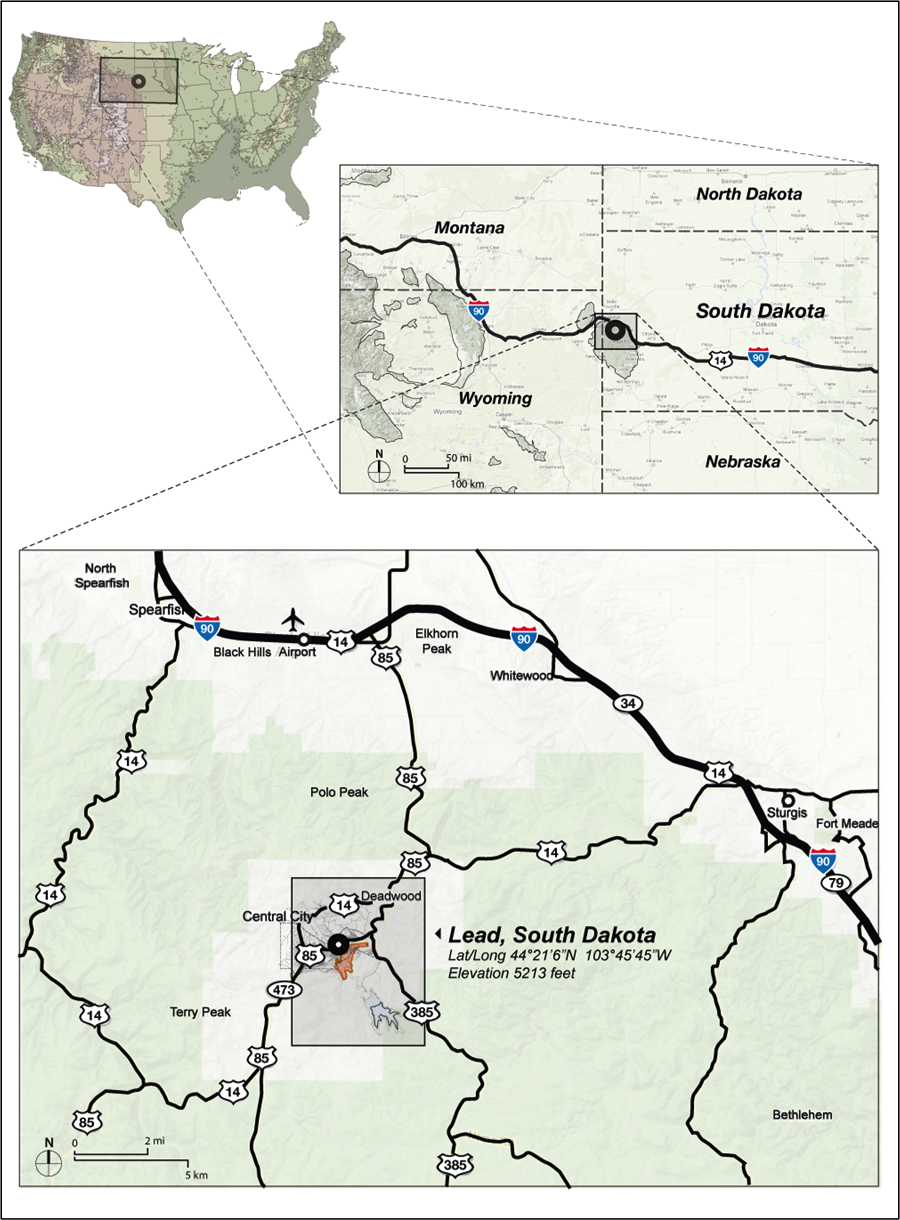
\includegraphics[width=0.8\textwidth]{regional-context}
\end{cdrfigure}


\begin{cdrfigure}[SURF Complex shown in the context of the city of Lead, South Dakota]{surf-complex}{SURF Complex shown in the context of the city of Lead, South Dakota, and the property remaining under ownership of Barrick. Area shown in yellow is a potential future expansion of the SDSTA property. [Dangermond Keane Architecture, Courtesy of SURF]}
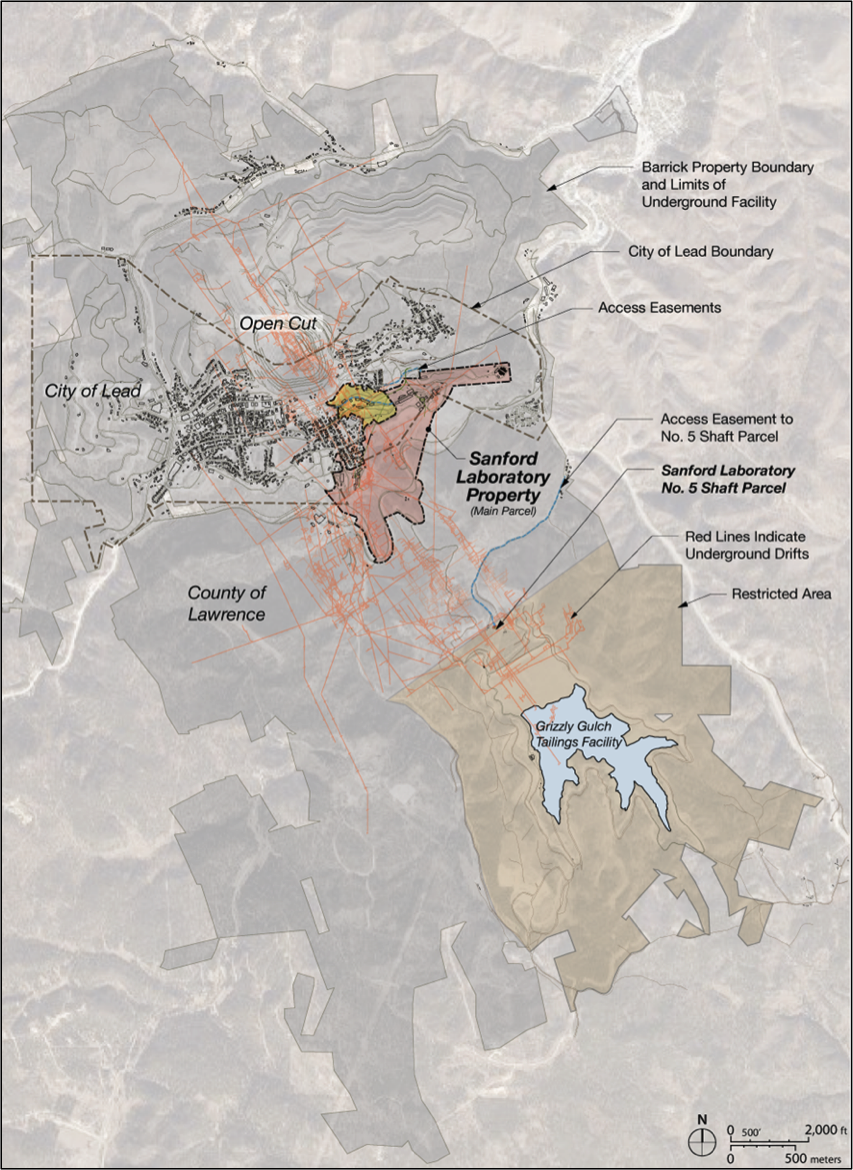
\includegraphics[width=0.8\textwidth]{rsurf-complex}
\end{cdrfigure}


%%%%%%%%%%%%%%%%%%%%%%%%%%%%%%%%%%%%%%%%%%%%%%%%%%%%%%%%%%%%%%%%%%%
\section{Existing  Site Conditions Evaluation}
\label{sec:fscf-site-cond-eval}

The facility conditions as of \fixme{year} were assessed by the architect/engineering firm HDR, as part of the DUSEL Preliminary Design to
evaluate the condition of existing facilities and structures on the Yates, and Ross Campuses.
They are documented in the DUSEL PDR, Section 5.2.4~\cite{dusel-pdr}. 
The portions of DUSEL's assessment pertinent to the LBNF Project are included here; they have been edited to reflect current activities and conditions. References to the DUSEL Project are from that time, and are now considered historic.

%Site and facility assessments were performed during DUSEL's Preliminary Design phase by HDR to . 

The HDR assessments reviewed the condition of buildings that were proposed for %continuing present 
continued use in their then-current function, new use, or potential demolition. Assessments for buildings were performed %in the categories of 
on their architectural, structural, mechanical/electrical/plumbing (MEP), civil, environmental, and historic aspects. Site assessments looked at %the categories that included 
civil, landscape, environmental, and historic aspects. Facility-wide utilities such as electrical, steam distribution lines, water and sewer systems were also assessed. In particular:

%The site and facility assessments outlined above were performed during DUSEL's Preliminary Design. 
\begin{itemize} 
\item Buildings proposed for reuse were evaluated through preliminary architectural and full structural, environmental, and historic assessments. 
\item Buildings proposed for demolition were evaluated through preliminary historic assessments.
\item Preliminary MEP assessments were performed on the Ross Substation, \#5 Shaft fan, Oro Hondo fan, Oro Hondo substation, and on the general site utilities for the Ross, Yates, and Ellison Campuses.
 \item The waste water treatment plant (WWTP) received preliminary architectural and structural assessments and a full MEP assessment.
 \item Preliminary civil assessments of the Kirk Portal site and Kirk to Ross access road were also completed.
 \end{itemize}

The assessment %evaluation 
was completed in three phases and the detailed reports are included in the appendices of the DUSEL PDR as:

\begin{itemize}
 \item Phase I Report, Site Assessment for Surface Facilities and Campus Infrastructure to Support Laboratory Construction and Operations (DUSEL PDR Appendix 5.E)
 \item Phase II Site and Surface Facility Assessment Project Report (DUSEL PDR Appendix 5.F)
 \item Phase II Roof Framing Assessment (DUSEL PDR Appendix 5.G)
     \end{itemize}


%%%%%%%%%%%%%%%%%%%%%%%%%%%%%%%%%%%%%%%%%%%%%%%%%%%%%%%%%%%%%%%%%%%
\section{Evaluation of Geology and Existing Excavations}
\label{sec:fscf-site-cond-geo}

%LBNF Far Site facilities are planned to be constructed at SURF which is being developed 
The accessible underground mine workings at SURF within the footprint of the former Homestake Gold Mine are extensive.  %located in Lead, South Dakota. 
Over the life of the gold mine, over 360 miles of drifts (tunnels) were mined, and shafts and winzes were sunk to gain access to depths in excess of 8,000 feet. A number of underground workings are being refurbished by SURF, and new experiments are being installed %developed 
at the 4850L, the same level as proposed for the LBNF underground facilities. Geotechnical investigations and initial geotechnical analyses were completed by Arup, USA \fixme{I see citation for lachel felice, not arup; cite both geotech and pdr?} for the DUSEL Preliminary Design and are described in detail in the DUSEL Preliminary Design Report~\cite{lachel-geotech, dusel-pdr}. Additional geotechnical investigation and analyses were performed, also by Arup, in 2014 specific to LBNF.  This section provides summaries of these two efforts, including work completed for DUSEL that is applicable to LBNF (the text is excerpted from the DUSEL PDR, Chapter 5 Section 3). Much of the work completed for the alternative detector technology considered during the DUSEL timeframe, a water Cherenkov detector (WCD), is also applicable to the current LBNF design at the 4850L.  


%%%%%%%%%%%%%%%%%%%%%%%%%%%%%%%%%%
\subsection{Geologic Setting}
\label{sec:fscf-site-cond-geo-set}

SURF is sited within a metamorphic complex containing the Poorman, Homestake, Ellison and Northwestern Formations (oldest to youngest), which are sedimentary and volcanic in origin. An amphibolite unit (Yates Member) is present within the lower known portions of the Poorman Formation. The LBNF %cavity has 
caverns have been located in the Poorman formation to isolate them from the remainder of the level. The layout adopted on the 4850L attempts to optimize the needs for ventilation isolation, access control, and orientation relative to the beamline.

%%%%%%%%%%%%%%%%%%%%%%%%%%%%%%%%%%
\subsection{Rock Mass Characteristics: LBNF}
\label{sec:fscf-site-cond-geo-rock}

Following a similar strategy as DUSEL, LBNF initiated a second geotechnical program in 2013 to evaluate the specific location under consideration and evaluate its appropriateness for the proposed design.  This was undertaken in two phases.  The first phase was a mapping of the existing spaces surrounding the proposed rock mass using both visual techniques and laser scanning to understand the rock mass and to inform the scope of the second phase.  The second phase included drilling of four HQ (2.5-in diameter) core holes ranging in length from 477 to 801 feet as well as two 6-in diameter core holes $\sim$30~ft each.  The smaller diameter cores were then evaluated for the following characteristics:

\begin{itemize}
 \item core recovery percent
 \item rock quality designation (RQD) percent
 \item rock type, including color, texture, degree of weathering, and strength
 \item mineralogy and presence of magnetic sulfides
 \item character of discontinuities, joint spacing, orientation, aperture
 \item roughness, alteration, and infill (if applicable)
\end{itemize}

Representative samples were selected from the overall core to test material strength and chemical characteristics. The geotechnical site investigations area on the 4850L, showing boreholes is presented in Figure~\ref{fig:core-loc}. 

The holes from which the smaller diameter core was removed were studied in several ways.  An absolute survey was conducted to allow the core holes to be plotted relative to cavern designs.  An optical televiewer was passed through each small hole to visualize the rock mass.  This technique allows visualization of foliation, joint openings, healed joints, and geological contact between rock types.  An acoustical imaging device was also used in one hole to complement the optical information.  The permeability of the rock was tested by pressurizing the small holes at various intervals to determine whether joints allowed for the flow of water outside of the holes (hydraulic conductivity).  In all cases, the hydraulic conductivity was well below what can be accomplished using manmade techniques such as grouting.   Two of the small holes were plugged and instrumented to determine whether water would flow into the holes over time.  This test found very low flow rates (.0013 -- .0087 gpm).  Ongoing evaluation of pressure build in these holes was inconclusive, as blast-induced fracturing near the existing drifts allow the holes to depressurize outside of the measurement capacity of the test instruments.

\begin{cdrfigure}[LBNF core locations and geological features]{core-loc}{LBNF core locations and geological features}
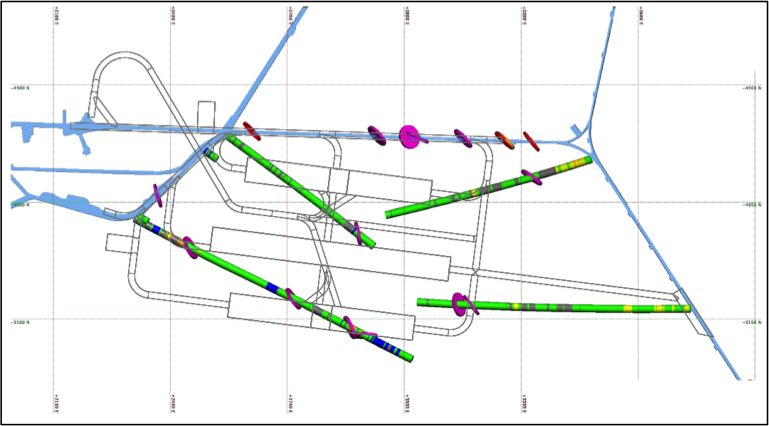
\includegraphics[width=0.8\textwidth]{core-loc}
\end{cdrfigure}

The larger (6-in) diameter cores and holes were used for strength and stress testing.  In situ stress was tested by drilling a smaller diameter hole first, then gluing a strain gauge at 30 -- 36 feet within the depth.  As the larger diameter core was removed, this strain gauge recorded the relaxation of the rock.  The removed core was re-drilled to provide smaller diameter samples at specific orientations for strength testing, as the strength of the material varies based on applied force direction relative to the foliation of the rock.  These samples were also tested for time-dependent movement. 

LBNF reviewed the analysis performed by Arup by enlisting industry leaders as part of a Neutrino Cavity Advisory Board (NCAB).  This board reviewed the %philosophy 
approach and results of the geotechnical investigation program as well as the preliminary excavation design.  Their conclusions indicated that no additional drilling would be required to provide design information for the project and the overall design approach was appropriate.  The board provided many recommendations that will %benefit the 
advance the design, 
for example, replacement of wire mesh with fiber-reinforced shotcrete in all excavations, reduction of the distance between caverns, and optimization of the ground support aimed at replacing cable support wherever possible. 


For further details, see Arup's Geotechnical Interpretive Report~\cite{arup-100-2011-3a}.

%%%%%%%%%%%%%%%%%%%%%%%%%%%%%%%%%%
\subsection{Geologic Conclusions}
\label{sec:fscf-site-cond-geo-concl}

Recovery of rock cores was performed along with geologic mapping to determine if discontinuities in the rock mass exist that could cause difficulties in the %construction 
excavation and maintenance of the planned caverns. In general, the proposed locations of the excavations %do not appear to be complicated by geologic structures that cause undue difficulties for construction. 
appear to be free of problematic structures. This information, along with measurement of in situ stresses, has allowed numerical modeling of the stresses associated with the anticipated excavations. A sample of some of the initial modeling %done 
is provided in Figure~\ref{fig:contour-stress-safety}.

\begin{cdrfigure}[Contour of stress safety factor]{contour-stress-safety}{Contour of stress safety factor indicating influences between caverns}
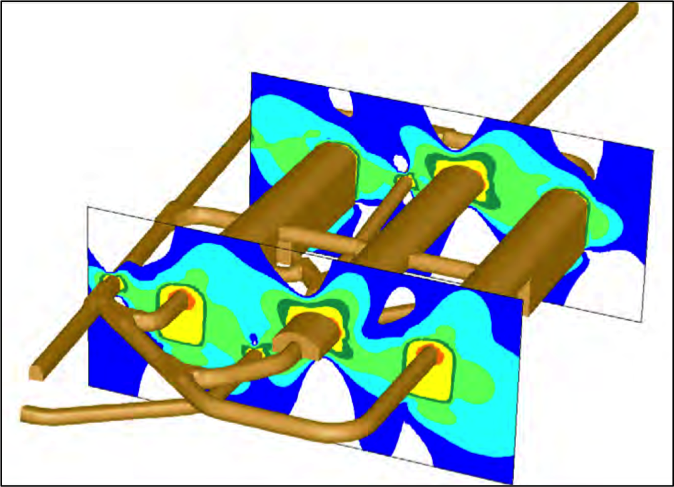
\includegraphics[width=0.8\textwidth]{contour-stress-safety}
\end{cdrfigure}


